\section{Cálculo Lambda Tipado}

El cálculo lambda es un modelo de computación turing completo basado en \textbf{funciones} introducido por \textbf{Alonzo Church}. Este modelo consiste en un conjunto de expresiones o terminos que representan abstracciones o aplicaciones de funciones y cuyos valores pueden ser determinados aplicando ciertas reglas sintacticas hasta obtener lo 	que se dice su forma normal, una expresión que, a falta de reglas no puede ser reducida de ninguna manera. En nuestro caso, estamos estudiando cálculo lambda tipado, es decir que habrá expresiones que, a pesar de estar bien formadas, no tendrán sentido.

\subsubsection{Expresiones de Tipos de \texorpdfstring{$\lambda^b$}{lambda b}}
El primer lenguaje lambda que usamos en la materia tiene dos \textbf{tipos} $Bool$ y $\sigma\rightarrow\theta$ que son los tipos de los valores booelanos y las funciones que van de un tipo $\sigma$ a un tipo $\theta$, respectivamente. Y lo notamos:
\begin{equation*}
	\sigma,\theta ~::=~ Bool ~|~ \sigma\rightarrow\theta
\end{equation*}

Una vez que definamos por completo el lenguaje lambda para estos dos tipos, esto es definir reglas de sintaxis, de tipado y de reducción de expresiones, vamos a extender el lenguaje con los naturales y, luego, con otros tipos de interés, como abstracciones de memoria y comandos.
\subsubsection{Términos de \texorpdfstring{$\lambda^b$}{lambda b}}
Ahora debemos definir los \textbf{términos} que nos permitirán escribir las expresiones válidas del tipado. Sea $\mathcal{X}$ un conjunto infinito enumerable de variables y $x\in\mathcal{X}$. Los \textbf{términos} de $\lambda^b$ están dados por:

\begin{equation*}
\begin{split}
    M, P, Q ~ ::&= ~ true \\
    & |~ false \\
    & |~ \lambdaIf{M}{P}{Q} \\
    & |~ \lambdaApp{M}{N} \\
    & |~ \lambdaAbs{x}{\sigma}{M} \\
    & |~ x
\end{split}
\end{equation*}

Esto significa que dados tres términos $M$, $P$ y $Q$, los términos válidos del lenguaje son:
\begin{itemize}
    \item $true$ y $false$ que representan las \textbf{constantes de verdad}.
    \item $ \lambdaIf{M}{P}{Q}$ que expresa el \textbf{condicional}.
    \item $\lambdaApp{M}{N}$ que indica la \textbf{aplicación} de la función denotada por el termino $M$ al argumento $N$.
    \item $\lambdaAbs{x}{\sigma}{M}$ que es una \textbf{función} (abstracción) cuyo parámetro formal es $x$ y cuyo cuerpo es $M$
    \item $x$, una \textbf{variable de términos}.
\end{itemize}

\subsubsection{Variables ligadas y libres}
Por como definimos el lenguaje, una variable $x$ puede ocurrir de dos formas: \textbf{libre} o \textbf{ligada}. Decimos que $x$ ocurre \textbf{libre} si no se encuentra bajo el alcance de una ocurrencia de $\lambda x$. Caso contrario ocurre ligada.

Por ejemplo:
$$\lambdaAbs{x}{Bool}{\lambdaIf{true}{\underbrace{x}_{ligada}}{\underbrace{y}_{libre}}} $$

Para conseguir las variables ligadas de una expresión, vamos a definir la función $FV$ que toma como parámetro una expresión y devuelve el conjunto de variables libres de la misma.

\begin{equation*}
\begin{split}
FV(x) &\equalDef {x} \\
FV(true) = FV(false) &\equalDef \phi \\
FV(\lambdaIf{M}{P}{Q}) &\equalDef FV(M)\cup FV(P)\cup FV(Q) \\
FV(\lambdaApp{M}{N}) &\equalDef FV(M)\cup FV(N) \\
FV(\lambdaAbs{x}{\sigma}{M}) &\equalDef FV(M) \backslash \{x\}
\end{split}
\end{equation*}

\subsubsection{Reglas de sustitución}

Una de las operaciones que podemos realizar sobre las expresiones del lenguaje es la \textbf{sustitución} que, dado un término $M$, sustituye todas las ocurrencias \textbf{libres} de una variable $x$ en dicho término por un término $N$. La notamos:

$$\replaceBy{M}{x}{N}$$

Esta operación nos sirve para darle semántica a la aplicación de funciones y es sencilla de definir, sin embargo debemos tener en cuenta algunos casos especiales.

\paragraph{$\alpha$-equivalencia} Dos terminos $M$ y $N$ que difieren solamente en el nombre de sus variables ligadas se dicen $\alpha$-equivalentes. Esta relación es una relación de equivalencia. Técnicamente, la sustitución está definida sobre clases de $\alpha$-equivalencia de términos


\paragraph{Captura de variables}\label{calculo_lambda:captura_variables} El primer problema se da cuando la sustitución que deseamos realizar sustituye una variable por otra con el mismo nombre que alguna de las variables ligadas de la expresión. Por ejemplo:
$$\replaceBy{(\lambdaAbs{z}{\sigma}{x})}{x}{z} = \lambdaAbs{z}{\sigma}{z}$$

En estos casos, si realizamos la sustitución cambiariamos el significado de la expresión (en el caso mostrado, estariamos convirtiendo la función constante que devuelve $x$ en la función identidad). Por esta razón debemos asegurarnos que cuando realizemos la operación $\replaceBy{\lambdaAbs{y}{\sigma}{M}}{x}{N}$, la variable ligada $y$ sea renombrada de tal manera que \textbf{no} ocurra libre en $N$.

\vspace*{5mm}
Entonces, teniendo en cuenta lo mencionado, definimos el comportamiento de la operación:

\begin{equation*}
\begin{split}
\replaceBy{x}{x}{N} &\equalDef N \\
\replaceBy{a}{x}{N} &\equalDef a \text{ si } a \in \{true,false\}\cup\mathcal{X}\backslash\{x\} \\
\replaceBy{(\lambdaIf{M}{P}{Q})}{x}{N} &\equalDef \lambdaIf{\replaceBy{M}{x}{N}}{\replaceBy{P}{x}{N}}{\replaceBy{Q}{x}{N}}\\
\replaceBy{(\lambdaApp{M_1}{M_2})}{x}{N} &\equalDef \lambdaApp{\replaceBy{M_1}{x}{N}}{\replaceBy{M_2}{x}{N}}\\
\replaceBy{(\lambdaAbs{y}{\sigma}{M})}{x}{N} &\equalDef \lambdaAbs{y}{\sigma}{\replaceBy{M}{x}{N}}~x\neq y,~y\notin~FV(N)
\end{split}
\end{equation*}

La condición $x\neq y,~y\notin~FV(N)$ está para que efectivamente no se produzca la situación mencionada en el parrafo anterior. Y \textbf{siempre} puede cumplirse, solo hay que renombrar las variables de manera apropiada.

\subsubsection{Árbol sintáctico}
Dada una expresión $M$, su árbol sintáctico es un árbol que tiene como raíz a $M$ y como hijos de la raíz a los árboles sintácticos de las expresiones que componen a $M$. Si $M$ no puede ser reducida, entonces, es el árbol trivial.

\begin{center}
	    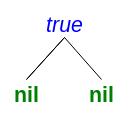
\includegraphics[scale=0.5, keepaspectratio=true]{imagenes/sintax_tree_true.png}
\end{center}
\subsection{Sistema de tipado}
El sistema de tipado es un sistema formal de deducción (o derivación) que utiliza axiomas y reglas de tipado para caracterizar un subconjunto de los términos. A estos términos los llamamos \textbf{términos tipados}.

Como dijimos, vamos a estudiar lenguajes de cálculo lambda tipado, por lo que para que una expresión sea considerada una expresión válida del lenguaje no solo debe ser sintácticamente correcta sino que debemos poder inferir su tipo a través del sistema de tipado que definamos. Y si no es posible inferir el tipo de una expresión con el sistema dado, entonces no la consideraremos una expresión válida del lenguaje.

\paragraph{Contexto de tipado}: Es un conjunto de pares $x_i:\sigma_i$, anotado $\Gamma = \{x_1:\sigma_1, \dots, x_n:\sigma_n\}$ que nos indica los tipos de cada variable de un programa.

Dado un contexto de tipado $\Gamma$, un \textbf{juicio de tipado} es una expresion $\judgeType{\Gamma}{M}{\sigma}$ que se lee ``el término M tiene tipo $\sigma$ asumiendo el contexto de tipado $\Gamma$''. 

\subsubsection{Axiomas de tipado de \texorpdfstring{$\lambda^b$}{lambda b}}

\begin{equation*}
\begin{gathered}
    \frac{}{\judgeType{\Gamma}{true}{Bool}}(\text{T-True}) \hspace*{2cm} \frac{}{\judgeType{\Gamma}{false}{Bool}}(\text{T-False})\hspace*{2cm} \\
    \vspace*{5mm} \\
    \frac{x:\sigma\in\Gamma}{\judgeType{\Gamma}{x}{\sigma}}(\text{T-Var})\hspace*{2cm}
\end{gathered}
\end{equation*}

\vspace*{5mm}
Los axiomas \textbf{T-True} y \textbf{T-False} nos dicen, que no importa el contexto en el que se encuentren los valores \textit{true} y \textit{false}, respectivamente, ambos valores serán de tipo \textit{Bool}. El axioma \textbf{T-Var}, nos dice que una variable libre $x$ es de $\sigma$ en un contexto $\Gamma$ entonces el par $x:\sigma$ se encuentra en $\Gamma$

\subsubsection{Reglas de tipado de \texorpdfstring{$\lambda^b$}{lambda b}}
\begin{equation*}
\begin{gathered}
\frac{\judgeType{\Gamma}{M}{Bool}\hspace*{5mm}\judgeType{\Gamma}{P}{\sigma}\hspace*{5mm}\judgeType{\Gamma}{Q}{\sigma}}{\judgeType{\Gamma}{\lambdaIf{M}{P}{Q}}{\sigma}}(\text{T-If}) \\
\vspace*{5mm} \\
\frac {\judgeType{\Gamma,x:\sigma}{M}{\tau}}
      {\judgeType{\Gamma}{\lambdaAbs{x}{\sigma}{M}}{\sigma\to\tau}}(\text{T-Abs})\hspace*{2cm}
\frac{\judgeType{\Gamma}{M}{\sigma\to\tau}\hspace*{5mm}\judgeType{\Gamma}{N}{\sigma}}{\judgeType{\Gamma}{\lambdaApp{M}{N}}{\tau}}(\text{T-App})
\end{gathered}
\end{equation*}

\vspace*{5mm}
\textbf{T-If} nos dice que si $\lambdaIf{M}{P}{Q}$ es de tipo $\sigma$ en $\Gamma$, entonces $M$ es de tipo $Bool$ y $P$ y $Q$ son de tipo $\sigma$ en $\Gamma$.

\textbf{T-Abs} indica que si $\lambdaAbs{x}{\sigma}{M}$ es de tipo $\sigma\to\tau$ en $\Gamma$, entonces $M$ es de tipo $\tau$ y $x$ en de tipo $\sigma$ en $\Gamma$.

\textbf{T-App} significa que si $\lambdaApp{M}{N}$ es de tipo $\sigma\to\tau$ en $\Gamma$, entonces $M$ es de tipo $\tau$ en el contexto $\Gamma, x:\sigma$. Este es el contexto formado por la unión disjunta entre $\Gamma$ y $x:sigma$, o en castellano, el contexto que remplaza el tipo de $x$ en $Gamma$ por $\sigma$.

\subsubsection{Resultados básicos}

Si $\judgeType{\Gamma}{M}{\sigma}$ puede derivarse usando los axiomas y reglas de tipados decimos que el juicio es \textbf{derivable}. Además, si el juicio se puede derivar para algún $\Gamma$ y $\sigma$, entonces decimos que $M$ es \textbf{tipable}.

\paragraph{Unicidad de tipos} Si $\judgeType{\Gamma}{M}{\sigma}$ y $\judgeType{\Gamma}{M}{\tau}$ son derivables, entonces $\sigma = \tau$

\paragraph{Weakening + Strengthening} Si $\judgeType{\Gamma}{M}{\sigma}$ es derivable y $\Gamma\cap\Gamma'$ contiene a todas las variables libres de $M$, entonces $\judgeType{\Gamma'}{M}{\sigma}$

\paragraph{Sustitución} Si $\judgeType{\Gamma,x:\sigma}{M}{\tau}$ y $\judgeType{\Gamma}{N}{\sigma}$ son derivables, entonces $\judgeType{\Gamma}{\replaceBy{M}{x}{N}}{\tau}$ es derivable.

\subsection{Semántica operacional}
Ya definimos cuales serán los términos y expresiones válidas de nuestro lenguaje. El siguiente paso, es definir algún mecanismo que nos permita inferir el significado o \textbf{valor} de un término. 

Para lograr este objetivo definimos lo que se llama \textbf{semántica operacional}, un mecanismo que interpreta a los \textbf{términos como estados} de una máquina abstracta y define una \textbf{función de transición} que indica, dado un estado, cual es el siguiente.

De esta forma, el significado de un término $M$ es el estado final que alcanza la máquina al comenzar con $M$ como estado inicial.

Tenemos dos formas de definir la semántica:
\begin{itemize}
    \item \textbf{Small-step}: La función de transición describe un paso de computación, descomponiendo los términos compuestos en términos más simples y especificando el orden el que deben ser reducidos.
    \item \textbf{Big-step} (o \textbf{Natural Semantics}): La función de transición, en un paso, evalúa el termino a su resultado.
\end{itemize}

Nosotros vamos a usar la primer opción. Y la formulamos a través de \textbf{juicios de evaluación} 
$$M\to N$$ que se leen ``\textit{el término M reduce, en un paso, al término N}''.

Para establecer el significado de estos juicios, vamos a definir \textbf{axiomas de evaluación} y \textbf{reglas de evaluación}. Los axiomas nos indicarán cuales juicios de evaluación son siempre derivables y las reglas nos dirán que juicios son derivables dado un contexto. Las reglas de la semántica asumen que las expresiones están bien tipadas.

\subsubsection{Expresiones Booleanas}\label{calculo_lambda:semantica:booleanas}
Los valores de las  expresiones booleanas son:
$$ V~::=~true~|~false$$
y son usados para reducir el término $\lambdaIf{M_1}{M_2}{M_3}$ mediante los siguientes axiomas:

\begin{equation*}
\frac{}{\lambdaIf{true}{M_1}{M_2} \to M_1}(\text{E-IfTrue})
\end{equation*}
\vspace*{5mm}
\begin{equation*}
\frac{}{\lambdaIf{false}{M_1}{M_2} \to M_2}(\text{E-IfFalse})
\end{equation*}
\vspace*{5mm}
\begin{equation*}
\frac{M_1\to M'_1}{\lambdaIf{M_1}{M_1}{M_2}\to\lambdaIf{M'_1}{M_1}{M_2}}(\text{E-If})
\end{equation*}

\vspace*{5mm}
Estas reglas nos indican que dado un término del tipo $\lambdaIf{M_1}{M_2}{M_3}$, si $M_1 = true$, entonces podemos remplazar la expresión por $M_2$, si $M_1=false$ entonces podemos remplazar la expresión por $M_3$ y si $M_1$ es una expresión reducible a $M'_1$, entonces podemos remplazar la expresión por $\lambdaIf{M'_1}{M_2}{M_3}$.

Con estas reglas definimos la estrategia de evaluación del condicional que se corresponde el orden habitual en lenguajes de programación:
\begin{enumerate}
    \item Primero evaluamos la guarda del condicional
    \item y una vez que la guarda sea un valor, evaluamos la expresión del \textit{then} o del \textit{else} según corresponda.
\end{enumerate}

\subsubsection{Propiedades}

\paragraph{Determinismo} Si $M\to M'$ y $M\to M''$ entonces $M' = M''$, esto quiere decir que el valor que representa $M$ no cambia con las reducciones que le apliquemos.

\paragraph{Valores en forma normal} Una \textbf{forma normal} es un término que no puede evaluarse más. Consideraremos que terminamos de evaluar un término cuando conseguimos su forma normal.

Todos los valores tiene una forma normal, sin embargo hay que tener en cuenta que como estamos definiendo un lenguaje tipado, habrá formas normales que no representen ningún valor.

\subsubsection{Evaluación en muchos pasos}
El juicio de \textbf{evualuación de muchos pasos} $\twoheadrightarrow$ es la clausura reflexiva, transitiva de $\to$. Es decir, la menor relación tal que:
\begin{enumerate}
    \item Si $M\to M'$, entonces $M\twoheadrightarrow M'$
    \item $M\twoheadrightarrow M$ para todo $M$
    \item Si $M\twoheadrightarrow M'$ y $M' \twoheadrightarrow M''$, entonces $M\twoheadrightarrow M''$
\end{enumerate}

\paragraph{Unicidad de formas normales} Si $M\twoheadrightarrow U$ y $M\twoheadrightarrow V$ con $U$ y $V$ formas normales, entonces $U = V$

\paragraph{Terminación}
Para todo $M$ existe una forma normal $N$ tal que $M\twoheadrightarrow N$


\subsection{Semántica operacional de \texorpdfstring{$\lambda^b$}{lambda b}}
En la sección \ref{calculo_lambda:semantica:booleanas} definimos el comportamiento de las expresiones booleanas, sin embargo, nos falta definir como reducir términos del tipo $\lambdaAbs{x}{\sigma}{M}$ y $\lambdaApp{M}{N}$.

Lo primero a tener en cuenta, es que vamos a considerar a los términos de $\lambdaAbs{x}{\sigma}{M}$ como valores, sin si $M$ es reducible o nó. Entonce, nuestro conjunto de valores del lenguaje sería:

$$ V  ~::=~ true~|~false~|~\lambdaAbs{x}{\sigma}{M}$$

Por lo que todo término bien tipado y cerrado (sin variables libres) evalúa a alguna de estos términos. Si es de tipo $Bool$ evalúa a $true$ o $false$, si es de tipo $\sigma\to\tau$ evalúa a $\lambdaAbs{x}{\sigma{M}}$
A las reglas y axiomas definidos para los tipos booleanos agregamos los siguientes:

\begin{equation*}
\frac{M_1\to M'_1}{\lambdaApp{M_1}{M_2} \to 
\lambdaApp{M'_1}{M_2}}(\text{E-App1}~ /~ \mu)
\end{equation*}
\vspace*{5mm}
\begin{equation*}
\frac{\lambdaApp{M_2}{M'_2}}{\lambdaApp{\lambdaAbs{x}{\sigma}{M}}{M_2} \to 
	\lambdaApp{\lambdaAbs{x}{\sigma}{M}}{M'_2}}(\text{E-App2}~/~v)
\end{equation*}	
\vspace*{5mm}
\begin{equation*}
\frac{}{\lambdaApp{\lambdaAbs{x}{\sigma}{M}}{V} \to 
	\replaceBy{M}{x}{V}}(\text{E-App2}~/~\beta)
\end{equation*}

\paragraph{Estado de error} Es un estado que \textbf{no es} un valor pero en el que la computación está trabada. Representa el estado en el cual el sistema de runtime de una implementación real generaría una excepción.

El sistema de tipado, nos garantiza que si un término cerrado está bien tipado entonces evalúa a un valor.


 \paragraph{Corrección}
La corrección de un término nos asegura dos cosas:	\textbf{Progreso} y \textbf{Preservación}.

El \textbf{progreso} asegura que si $M$ es un término cerrado y bien tipado, entonces $M$ es un valor o existe $M'$ tal que $M\to M'$. En otras palabras, nos asegura que la evaluación no puede trabarse para términos cerrados y bien tipados que no son valores. Y si un programa termina, entonces nos devuelve un valor.

La \textbf{preservación} asegura que la evaluación de un término $M$ preserva tipos. Es decir, no importa cuanta veces se reduzca $M$, el término resultante siempre es del tipo original.

$$\text{Si } \judgeType{\Gamma}{M}{\sigma} \text{ y } M\to N \text{ entonces } \judgeType{\Gamma}{N}{\sigma}$$	

